\documentclass[tikz,border=5pt]{standalone}
\usepackage[UTF8]{ctex}
\usepackage{amsmath,amssymb}
\usetikzlibrary{arrows.meta,calc,decorations.markings}
\tikzset{>=Stealth,line cap=round,line join=round,
wall/.style={black!75,very thick},
flow/.style={blue!70!black,thick},
directed/.style={postaction={decorate},decoration={markings,mark=at position .72 with{\arrow{Stealth}}}},
aux/.style={black!50,dashed,thin},
dim/.style={black!65,<->,thin},
dot/.style={circle,fill=black,inner sep=1.6pt}}
\begin{document}
% 1. Two distinct planar domains. Paths are schematic and stop at first contact.
\begin{tikzpicture}[font=\small,x=1cm,y=1cm]
\begin{scope}
\fill[blue!3](-3.35,0)rectangle(3.35,2.3);
\draw[wall](-3.5,0)--(3.5,0);
\draw[->](0,-.25)--(0,2.6)node[above]{$y$};
\draw[->](3.5,0)--(4,0)node[right]{$x$};
\node[below]at(-2.4,0){长城：首次触及即获救};
\coordinate(S)at(0,1.4);
\draw[green!40!black,thick,->](S)--(.55,1.72)--(.3,1.1)--(1.15,1.25)--(.85,.75)--(1.75,.95)--(2.45,.42)--(2.1,0);
\node[dot]at(S){};\node[above left]at(S){$S=(0,l)$};
\node[dot]at(2.1,0){};\node[below]at(2.1,0){$X_{\tau_0}$};
\draw[dim](-.72,0)--(-.72,1.4)node[midway,left]{$l$};
\node[anchor=east]at(-3.55,2.1){(a)};
\end{scope}
\begin{scope}[shift={(0,-4.1)}]
\fill[blue!3](-3.35,0)rectangle(3.35,2.5);
\draw[wall](-3.5,0)--(3.5,0);
\draw[red!65!black,very thick](-3.5,2.5)--(3.5,2.5);
\node[below]at(-2.05,0){长城：获救};
\node[above]at(-2.15,2.5){异鬼：终止};
\coordinate(S2)at(0,1);
\draw[green!40!black,thick,->](S2)--(-.5,1.3)--(-.9,.55)--(-1.45,.75)--(-2.2,0);
\draw[red!65!black,thick,->](S2)--(.6,.7)--(1.2,1.5)--(1.7,1.25)--(2.2,2.1)--(2.7,2.5);
\node[dot]at(S2){};\node[above]at(S2){$(0,l)$};
\draw[aux](.25,1)--(3.62,1);
\draw[dim](3.8,0)--(3.8,1)node[midway,right]{$l$};
\draw[dim](3.8,1)--(3.8,2.5)node[midway,right]{$h-l$};
\draw[dim](-3.8,0)--(-3.8,2.5)node[midway,left]{$h$};
\node[anchor=east]at(-3.55,2.9){(b)};
\end{scope}
\end{tikzpicture}
% 2. A single local isotropic step, not a global deterministic path.
\begin{tikzpicture}[font=\small]
\coordinate(O)at(0,0);
\pgfmathsetmacro{\xx}{1.8*cos(34)}
\pgfmathsetmacro{\yy}{1.8*sin(34)}
\coordinate(P)at(\xx,\yy);
\draw[gray!55,thick](O)circle(1.8);
\draw[->](-2.25,0)--(2.5,0)node[right]{$\Delta x$};
\draw[->](0,-2.05)--(0,2.35)node[above]{$\Delta y$};
\draw[flow,->](O)--(P)node[midway,above,sloped]{$a$};
\draw[aux](P)--(\xx,0);
\draw[aux](P)--(0,\yy);
\draw[blue!65!black](.55,0)arc(0:34:.55);
\node at(.81,.2){$\varphi$};
\node[dot]at(O){};\node[below left]at(O){$(x,y)$};
\node[dot]at(P){};\node[above right]at(P){下一位置};
\draw[dim](0,-.35)--(\xx,-.35)node[midway,below]{$a\cos\varphi$};
\draw[dim](\xx+.38,0)--(\xx+.38,\yy)node[midway,right]{$a\sin\varphi$};
\end{tikzpicture}
% 3. Exact cumulative-flow streamlines: circles through the source and its image.
\begin{tikzpicture}[font=\small,x=.85cm,y=.85cm]
\fill[gray!5](-5.3,-2.7)rectangle(5.3,0);
\draw[wall](-5.3,0)--(5.3,0);
\draw[->](0,-2.7)--(0,3.25)node[above right]{$y$};
\draw[->](5.3,0)--(5.7,0)node[right]{$x$};
\node[below left]at(-5.3,0){$y=0$};
\foreach \a in {-2,-.8,0,.8,2}{
\pgfmathsetmacro{\rr}{sqrt(\a*\a+4)}
\pgfmathsetmacro{\tt}{atan2(2,-\a)}
\draw[flow,directed]plot[domain=\tt:0,variable=\ang,samples=81]({\a+\rr*cos(\ang)},{\rr*sin(\ang)});
\draw[flow,directed]plot[domain=\tt:180,variable=\ang,samples=81]({\a+\rr*cos(\ang)},{\rr*sin(\ang)});
}
\coordinate(S)at(0,2);\coordinate(M)at(0,-2);\coordinate(P)at(2.7,0);
\draw[aux](S)--(P)node[pos=.77,above right,inner sep=1pt]{$r_+$};
\draw[aux](M)--(P)node[pos=.58,below right]{$r_-$};
\fill[blue!70!black](S)circle(.07);
\fill[red!70!black](M)circle(.07);
\node at(-1.1,3.55){$S=(0,l)$};
\draw[aux](-.6,3.35)--(-.04,2.08);
\node[below left]at(M){$S^*=(0,-l)$};
\node[right]at(.12,-2){负镜像源};
\node[dot]at(P){};\node[below right,inner sep=1pt]at(P){$P=(x,0)$};
\draw[red!65!black,->,thick](P)--(2.7,-.85)node[right]{$\boldsymbol n=-\boldsymbol e_y$};
\end{tikzpicture}
% 4. Cauchy density: x/l horizontally; l f vertically with a plotting scale 4.5.
\begin{tikzpicture}[font=\small,x=1cm,y=1cm]
\draw[->](-4.6,0)--(4.7,0)node[right]{$x/l$};
\fill[blue!9](-1,0)--plot[domain=-1:1,variable=\u,samples=101](\u,{4.5/(pi*(1+\u*\u))})--(1,0)--cycle;
\draw[->](0,0)--(0,1.95)node[above]{$lf(x)$};
\draw[flow,very thick]plot[domain=-4.4:4.4,variable=\u,samples=221](\u,{4.5/(pi*(1+\u*\u))});
\draw[aux](-1,0)--(-1,{4.5/(2*pi)})--(1,{4.5/(2*pi)})--(1,0);
\node[below]at(-1,0){$-1$};\node[below]at(1,0){$1$};\node[below left]at(0,0){$0$};
\draw[gray!65](-.06,{4.5/pi})--(.06,{4.5/pi});
\node[anchor=east]at(-.12,{4.5/pi}){$1/\pi$};
\draw[gray!65](-.06,{4.5/(2*pi)})--(.06,{4.5/(2*pi)});
\node[anchor=east,fill=white,inner sep=1pt]at(-.12,{4.5/(2*pi)}){$1/(2\pi)$};
\node[align=center]at(2.8,1.45){中心区间概率\\$P(|X_{\tau_0}|<l)=1/2$};
\end{tikzpicture}
% 5. Planar source-sheet analogy for integrated lower/upper flux only.
\begin{tikzpicture}[font=\small,x=1cm,y=1cm]
\draw[wall](-3.3,0)--(3.3,0);
\draw[wall](-3.3,3.8)--(3.3,3.8);
\draw[blue!65!black,densely dotted,very thick](-3.3,1.4)--(3.3,1.4);
\foreach \x in {-2.6,-1.3,0,1.3,2.6}{
\draw[flow,->](\x,1.25)--(\x,.15);
\draw[flow,->](\x,2.3)--(\x,2.9416667);
}
\node[below]at(0,0){下板：$y=0$，$P_b$};
\node[above]at(0,3.8){上板：$y=h$，$P_t$};
\node[right,fill=white,inner sep=1pt]at(3.35,1.4){单位源面};
\node[fill=white,inner sep=1pt]at(.55,.65){$E_b$};
\node[fill=white,inner sep=1pt]at(.55,2.6){$E_t$};
\draw[dim](-3.65,0)--(-3.65,1.4)node[midway,left]{$l$};
\draw[dim](-3.65,1.4)--(-3.65,3.8)node[midway,left]{$h-l$};
\node at(0,-.9){$E_b l=E_t(h-l),\qquad P_b+P_t=1$};
\end{tikzpicture}
% 6. Exponential map: lower boundary -> positive real axis, upper -> negative.
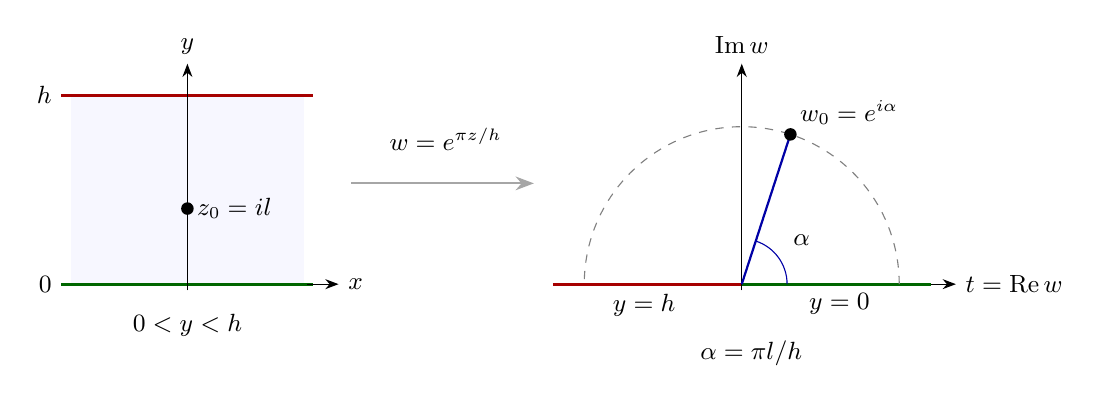
\begin{tikzpicture}[font=\small,x=.8cm,y=.8cm]
\begin{scope}
\fill[blue!3](-1.85,0)rectangle(1.85,3);
\draw[green!40!black,very thick](-2,0)--(2,0);
\draw[red!65!black,very thick](-2,3)--(2,3);
\draw[->](0,-.1)--(0,3.5)node[above]{$y$};
\draw[->](1.9,0)--(2.4,0)node[right]{$x$};
\node[dot]at(0,1.2){};\node[right]at(0,1.2){$z_0=il$};
\node[left]at(-2,0){$0$};\node[left]at(-2,3){$h$};
\node at(0,-.65){$0<y<h$};
\end{scope}
\node[align=center]at(4.1,2.3){$w=e^{\pi z/h}$};
\draw[gray!70,->,thick](2.6,1.6)--(5.5,1.6);
\begin{scope}[shift={(8.8,0)}]
\draw[red!65!black,very thick](-3,0)--(0,0);
\draw[green!40!black,very thick](0,0)--(3,0);
\draw[->](3,0)--(3.4,0)node[right]{$t=\operatorname{Re}w$};
\draw[->](0,-.1)--(0,3.5)node[above]{$\operatorname{Im}w$};
\coordinate(W)at({2.5*cos(72)},{2.5*sin(72)});
\draw[aux](2.5,0)arc(0:180:2.5);
\draw[blue!65!black,thick](0,0)--(W);
\draw[blue!65!black](.72,0)arc(0:72:.72);
\node at(.95,.7){$\alpha$};
\node[dot]at(W){};\node[above right]at(W){$w_0=e^{i\alpha}$};
\node[below]at(-1.55,0){$y=h$};
\node[below]at(1.55,0){$y=0$};
\node at(.15,-1.1){$\alpha=\pi l/h$};
\end{scope}
\end{tikzpicture}
\end{document}
